\documentclass[a4paper,12pt]{article} % Tipo de documento y tamaño de letra.
\usepackage[utf8]{inputenc} % Para que reconozca caracteres especiales como tildes.
\usepackage[spanish, es-nodecimaldot]{babel} % Para definir el idioma y el formato de fechas en español.
\usepackage{amsmath, amssymb} % Paquetes para símbolos y ecuaciones avanzadas (Para hacer una ecuación con un recuadro).
\usepackage{ragged2e} % Para justificar textos.
\usepackage{multicol} % Para crear columnas.
\usepackage{slashed} % Para generar números o variables canceladas (Una línea diagonal sobre el número o variable).
\usepackage{graphicx} % Paquete para poner graficas.
\usepackage{float} % Para poder dejar la imagen en un punto fijo del documento.
\usepackage{longtable} % Para tablas largas.
\usepackage{cancel} % Para hacer cancelaciones en medio de operaciones.
\usepackage{xcolor} % Para el color y esas cosas.
\usepackage{apacite} % Paquete para citas APA.
\usepackage{fancyhdr} % Para personalizar encabezados y pies de página.
\usepackage{geometry} % Para ajustar márgenes.
\usepackage{setspace} % Para ajustar el interlineado.
\usepackage{natbib} % Para manejar las citas y que no queden pegadas y feas :P.
\usepackage{hyperref} % Para que los enlaces funcionen con su URL.
\usepackage[version=4]{mhchem}  % Versión recomendada para mayor funcionalidad.
\usepackage{chemfig} %También para hacer estructuras químicas.
\usepackage{array} % Para mejor control de las columnas.
\usepackage{siunitx} % Para unidades físicas.
\usepackage{tabularx}
\usepackage[table]{xcolor}
\usepackage{booktabs}

\pagestyle{fancy}
\fancyhf{} % Limpia encabezados y pies de página predeterminados
\fancyhead[L]{\textbf{LABORATORIO.}} % Encabezado izquierdo
\fancyhead[R]{\textbf{ELECTROMAGNETISMO II.}} % Encabezado derecho
\fancyfoot[C]{\thepage} % Número de página en el centro del pie

\geometry{headheight=12.96115pt, top=1in, bottom=1in, left=1in, right=1in}
\begin{document}


\begin{figure}[H]
	\centering
	
\includegraphics[width=0.5\textwidth]{Unir.jpg}
\end{figure}

\vspace{\baselineskip}


\begin{center}
	\textbf{\Large } \\[0.3cm]
	\vspace{\baselineskip}
	\textbf{} \\[0.4cm]
	\textbf{Grado en Física.} \\[0.8cm]
	\textbf{Liz Ángel Núñez Torres.} \\[1 cm]
	\textbf{Universidad Internacional de La Rioja.} \\[1 cm]
	\textbf{1 de Mayo 2026.}
\end{center}

\newpage
\tableofcontents

\newpage

\section{Carga positiva en el centro de la pantalla.}

\begin{figure}[H]
	\centering
	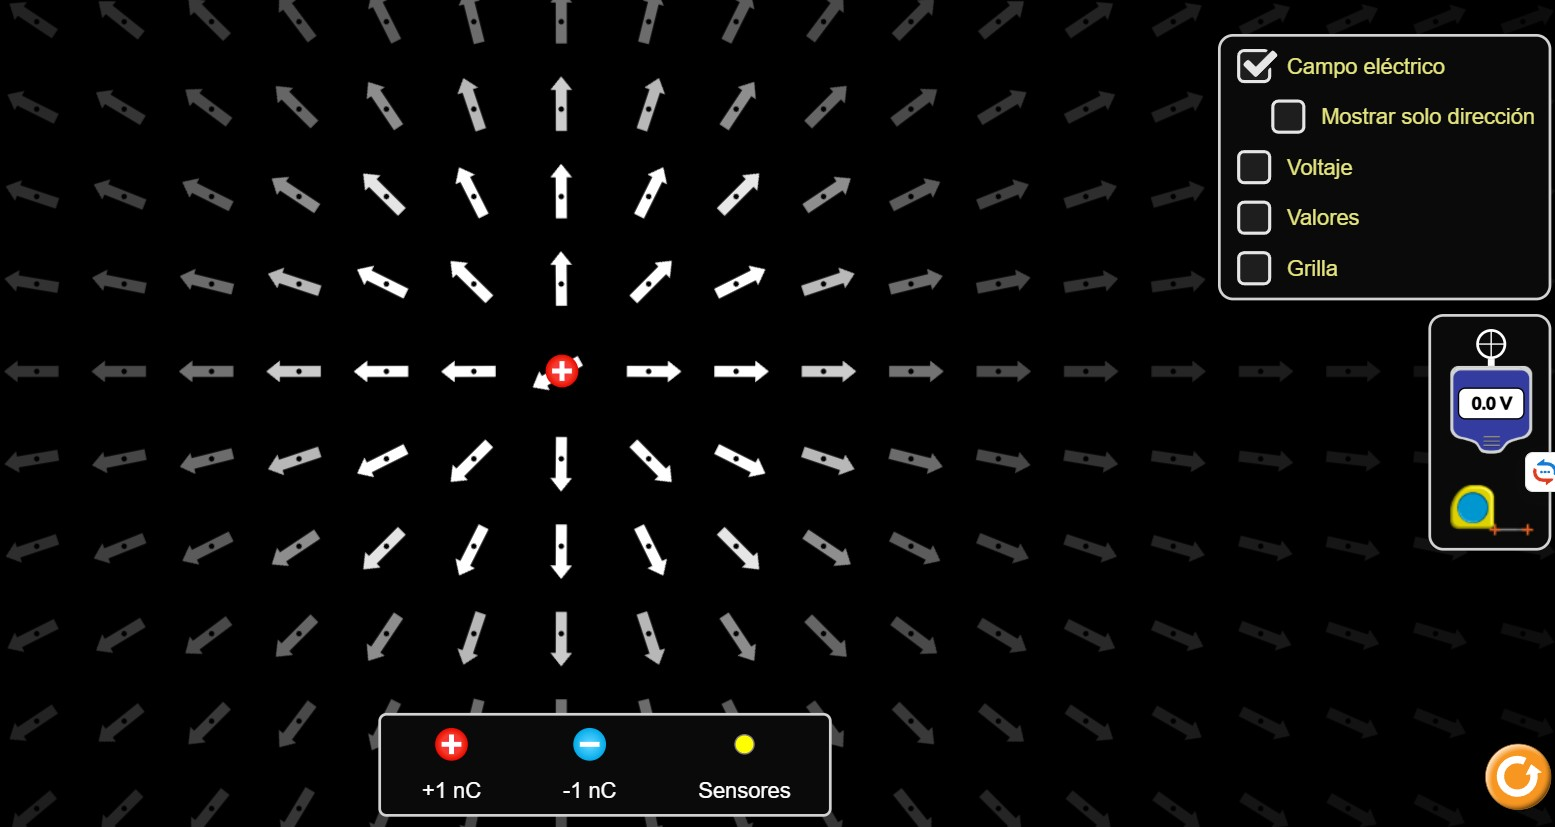
\includegraphics[width=0.9\textwidth]{fig1.jpg}
\end{figure}

\vspace{\baselineskip}

\subsection{¿Esta carga actúa como fuente o sumidero de campo eléctrico?}

\begin{figure}[H]
	\centering
	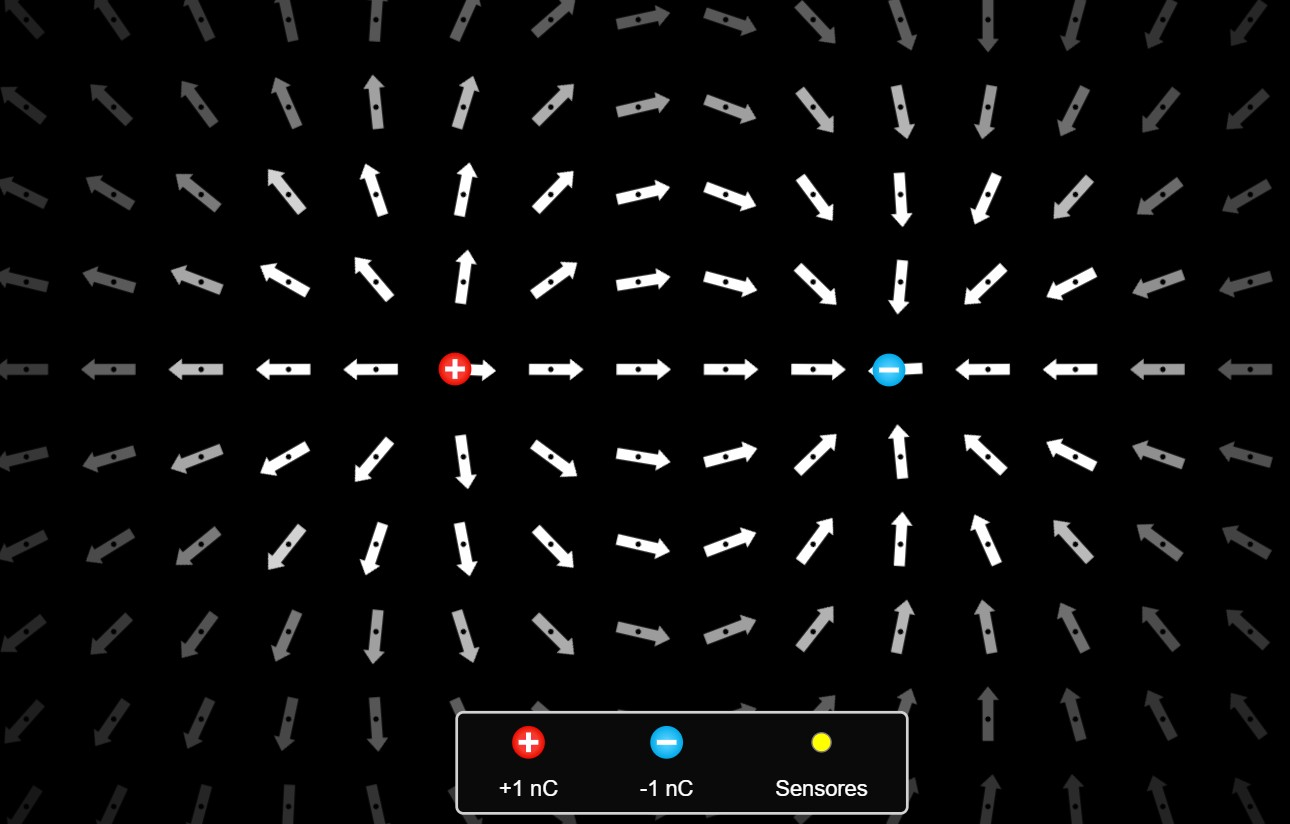
\includegraphics[width=0.9\textwidth]{fig2.jpg}
\end{figure}

\begin{itemize}
    \item Cuando tenemos dos cargas como en nuestro caso, \(+1 \, nC\) y \(-1 \, nC\) la \textbf{carga positiva} funciona como fuente, porque las líneas del campo salen en sentido radial hacia fuera. En el caso de la \textbf{carga negativa} funciona como sumidero, las líneas entran hacia la carga.
\end{itemize}


\vspace{\baselineskip}
\subsection{¿Qué representan las flechas que están dibujadas en la pantalla?}
\vspace{\baselineskip}

\begin{itemize}
    \item \begin{justify}
    Representa los vectores del campo eléctrico en diferentes puntos del espacio, donde cada fecha representa la dirección y sentido de la fuerza que experimentaría una carga prueba positiva si se colocara en ese punto.
        \end{justify}
\end{itemize}


\vspace{\baselineskip}
\subsection{¿Por qué son más brillantes las flechas cerca de la carga?}

\begin{itemize}
    \item Son más brillantes porque representan la magnitud del campo, cuando más brillante el campo es más fuerte, esto sucede por la \textbf{Ley de Coulomb} \(E = k\frac{|q|}{r^2}\) y disminuye con \(\frac{1}{r^2}\).
\end{itemize}

\vspace{\baselineskip}

\subsection{¿Qué representa la flecha roja?}

\begin{figure}[H]
	\centering
	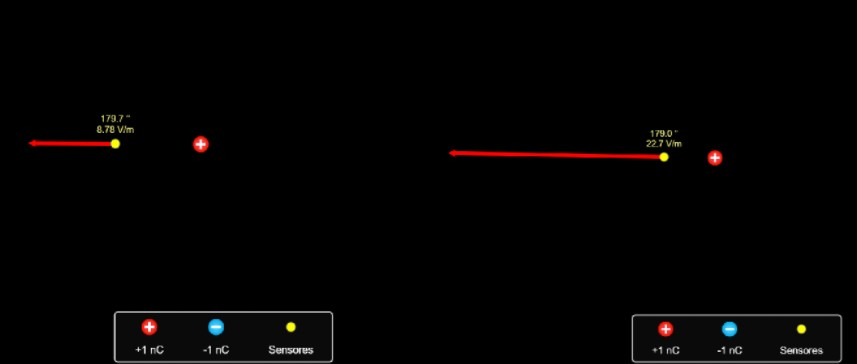
\includegraphics[width=0.9\textwidth]{fig3.jpg}
\end{figure}


\begin{itemize}
    \item La flecha roja representa el vector que genera el campo, su dirección, sentido y magnitud varian al poner el sensor más cerca o lejos de la carga.
\end{itemize}

\vspace{\baselineskip}

\subsection{¿Cuáles son las unidades en las que se mide el campo eléctrico?}

\begin{itemize}
    \item Las unidades son \textbf{N/C} Newton por Coulomb, aunque en el programa usamos su equivalencia \textbf{V/m} voltios por metro.
\end{itemize}


\vspace{\baselineskip}
\subsection{¿Cuál es el máximo valor de campo eléctrico en este experimento?}

\begin{figure}[H]
	\centering
	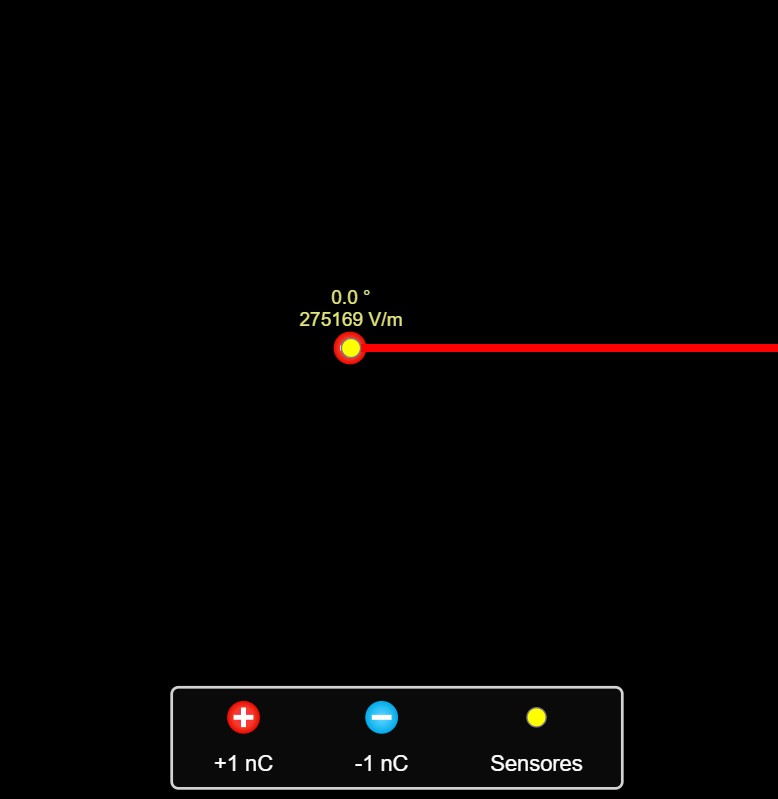
\includegraphics[width=0.7\textwidth]{fig4.jpg}
    \caption{Valor máximo del campo en nuestro experimento.}
\end{figure}


\vspace{\baselineskip}
\subsection{¿Por qué la flecha crece al acercarse a la carga positiva y decrece al alejarse?}

\begin{itemize}
    \item Esto sucede por la \textbf{Ley de Coulomb} \(E = k\frac{|q|}{r^2}\) y disminuye con \(\frac{1}{r^2}\) donde \(r\) representa la distancia.
\end{itemize}

\vspace{\baselineskip}

\newpage

\section{Mediciones del campo eléctrico.}

\begin{justify}
    Realice, por lo menos, diez mediciones de campo eléctrico para, posteriormente, graficar la dependencia respecto a la distancia. Compare las mediciones obtenidas por la simulación con las predicciones teóricas.
\end{justify}

\subsection{Mediciones.}
\begin{itemize}
    \item Realizaremos 10 mediciones partiendo de \(4 \, \mathrm{cm}\) hasta \(2.2 \, \mathrm{cm}\) en intervalos de \(2 \, \mathrm{cm}\).
\end{itemize}

\begin{figure}[H]
	\centering
	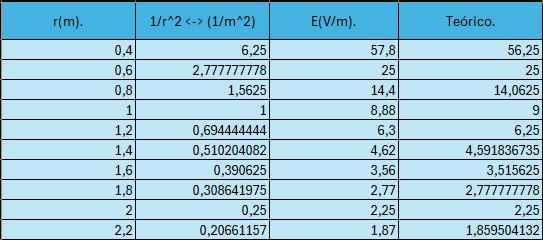
\includegraphics[width=0.9\textwidth]{fig5.jpg}
    \caption{Donde \textbf{r(m)} es la distancia y \textbf{E(V/m)} el campo medido en ese punto. }
\end{figure}

\begin{justify}
    En nuestra tabla, la columna \textbf{(\(1/r^2 (1/m^2)\))} representa la distancia de disminución del campo y \textbf{Teórico} representa las predicciones teóricas usando la \textbf{Ley de Coulomb}.
\end{justify}

\subsection{Grafica de la dependencia respecto a la distancia.}

\begin{figure}[H]
	\centering
	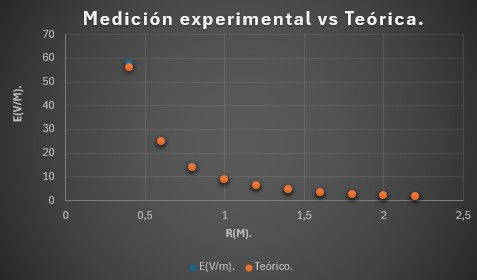
\includegraphics[width=0.7\textwidth]{fig6.jpg}
    \caption{Comparación entre las mediciones obtenidas por la simulación y la teórica.}
\end{figure}

\subsection{¿Qué valores piensa que obtendría si en lugar de una simulación se realiza un experimento?}

\begin{justify}
    Los valores obtenidos por medio de un experimento en un laboratorio estarían sujetos a un grado de error similar al expuesto en la simulación, siendo estos corregidos y analizados si usamos los fundamentos teóricos para hallar los resultados exactos.
\end{justify}

\section{Carga negativa.}

\begin{figure}[H]
	\centering
	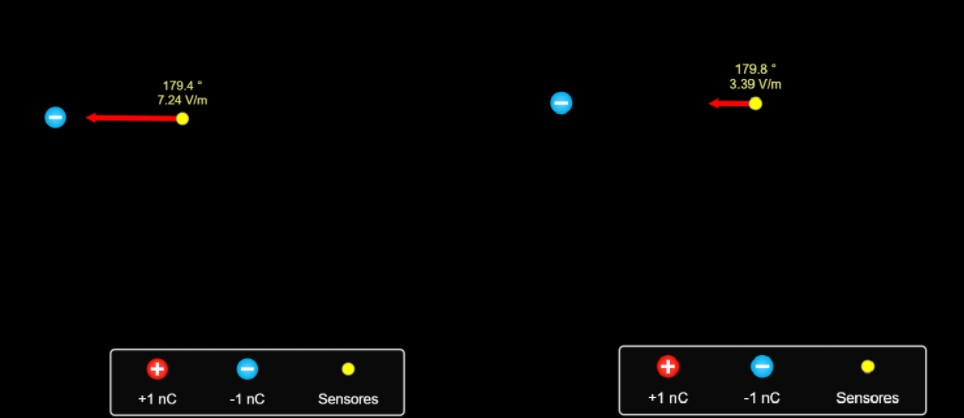
\includegraphics[width=0.9\textwidth]{fig7.jpg}
\end{figure}
\vspace{\baselineskip}

\subsection{¿La flecha roja tiene la misma dirección del campo? ¿Por qué?}

\begin{justify}
    Esto sucede porque el sensor representa la medida visual del vector al campo eléctrico en su posición, al cambiar de carga pasamos de una fuente a un sumidero lo que genera un cambio de sentido, no de dirección, por tanto la magnitud y sentido que refleja el sensor es un esbozo visual para la fuerza (Atractiva o repulsiva).
\end{justify}

\section{Hilo cargado positivamente.}

\begin{figure}[H]
	\centering
	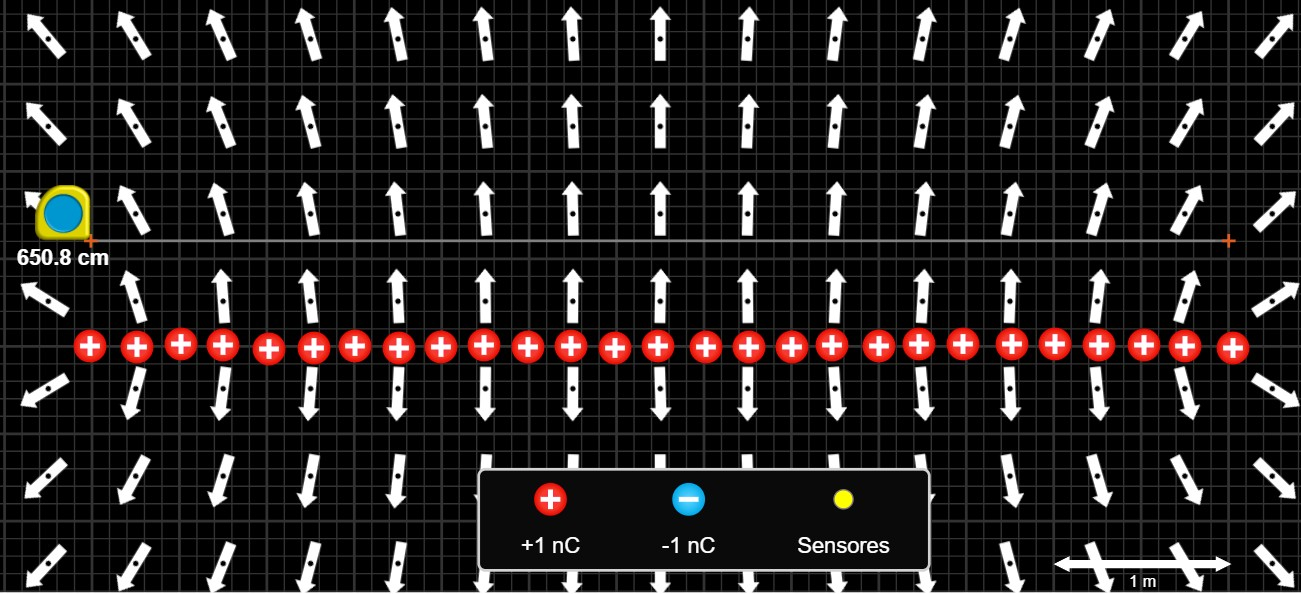
\includegraphics[width=0.69\textwidth]{fig8.jpg}
    \caption{Hilo cargado positivo de longitud de 6.50 m.}
\end{figure}
\vspace{\baselineskip}

\subsection{¿Qué disposición toman las flechas en el espacio? ¿Por qué?}

\begin{justify}
    Las flechas forman una simetría horizontal, donde apuntan hacia afuera debido a las cargas positivas que componen el hilo. Debido al principio de superposición, cada carga genera un campo que sale radialmente de ella, es la suma de los campos ocasionados por cada carga la que produce la simetría.
\end{justify}


\subsection{¿Qué ocurre cerca de las cargas que están en los extremos?}

\begin{justify}
    Las flechas se curvan ligeramente debido a la repulsión de las cargas contiguas. Además el campo medido por nuestro medidor en ese punto presenta una diminución en la fuerza repulsiva que la presentada paralelamente al hilo.
\end{justify}

\subsection{¿Qué rol juega la simetría en este experimento?}


\begin{justify}
    Presenta un papel importante dado que facilita las mediciones, la simetría nos dice por ejemplo que el efecto de los bordes (mencionado anteriormente) son iguales en ambos extremos y que las mediciones que tomemos delante o detrás del hilo van a presentar un sentido opuesto pero una misma dirección y fuerza electrica.
\end{justify}


\subsection{Mediciones.}


\begin{figure}[H]
	\centering
	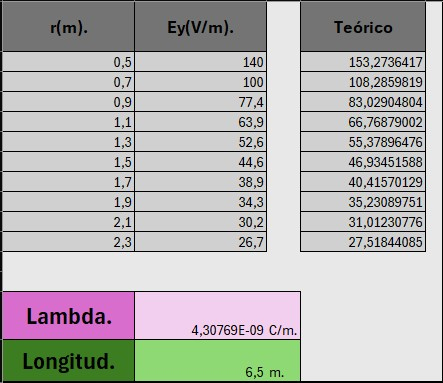
\includegraphics[width=0.69\textwidth]{fig9.jpg}
    \caption{Tabla de mediciones desde 5 cm hasta 23 cm en intervalos de 2 cm.}
\end{figure}

\begin{justify}
    En nuestra tabla, tenemos también la medición de lambda \(\lambda\) y la longitud del hilo cargado, cabe resaltar que nuestra medición parte desde la mitad de la longitud, \(\mathbf{3.25} \, \mathrm{cm}\).
\end{justify}

\subsection{Comparación de mediciones.}

\begin{figure}[H]
	\centering
	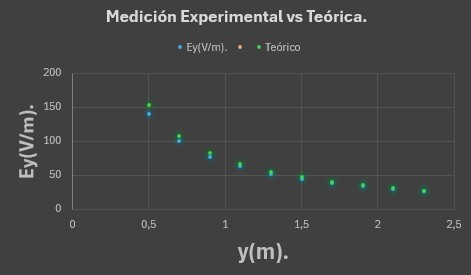
\includegraphics[width=0.8\textwidth]{fig10.jpg}
    \caption{Gráfica de comparación entre los datos obtenidos en la simulación y el teórico.}
\end{figure}

\subsection{Comportamiento del campo creado por el hilo cargado.}

\begin{justify}
    No se comportan de la misma forma dado que la dependencia radial generado por el hilo de carga es: \[\frac{1}{r}.\]  También la simetría es distinta, en un punto esta sería esférica y en un hilo es cilíndrica.
\end{justify}


\newpage

\section{Simulador del campo Magnético.}

\begin{justify}
    Realiza una tabla donde se registre el valor de la intensidad que introduces y el valor de la fuerza obtenido. Con estos valores haz una tabla:
\end{justify}

\begin{figure}[H]
	\centering
	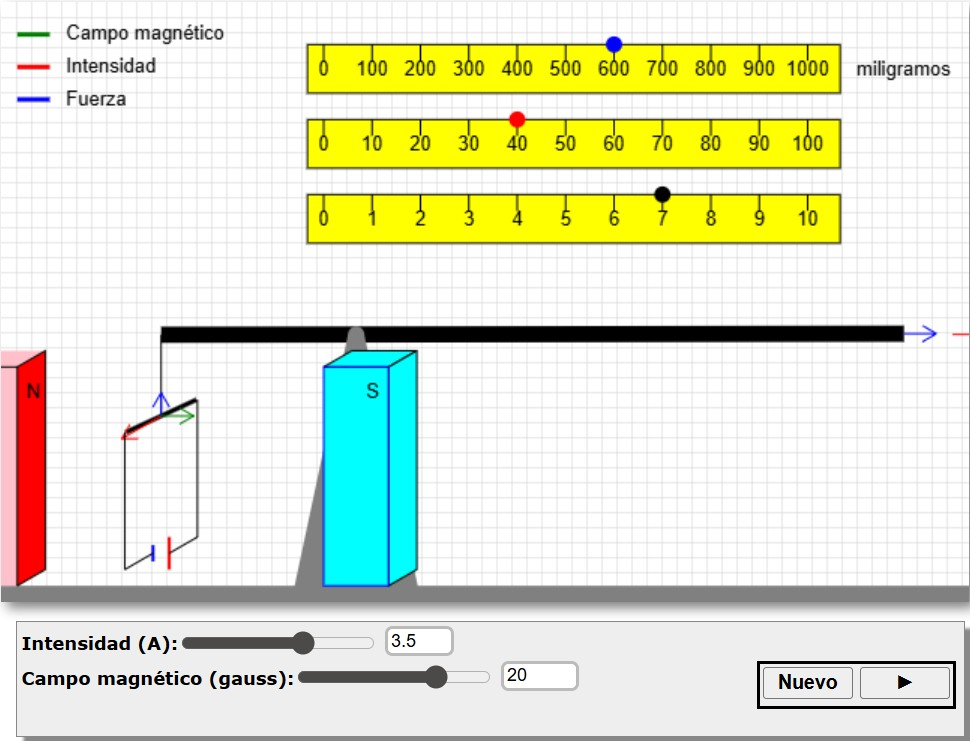
\includegraphics[width=0.9\textwidth]{fig12.jpg}
    \caption{Empezamos la medición con \textbf{intensidad(A) = 3.5} y masa aparente de \textbf{647 mg.}}
\end{figure}

\subsection{Tabla de medición.}

\begin{figure}[H]
	\centering
	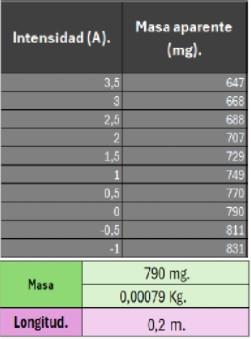
\includegraphics[width=0.5\textwidth]{fig11.jpg}
    \caption{Medición de la masa aparente a diferentes intensidades sabiendo que nuestra masa sin interferencia es de \textbf{790 mg} - \( \mathbf{7.9 \times 10^{-4} \mathrm{Kg}}. \)} 
\end{figure}

\subsection{Obtención de los datos.}

\begin{figure}[H]
	\centering
	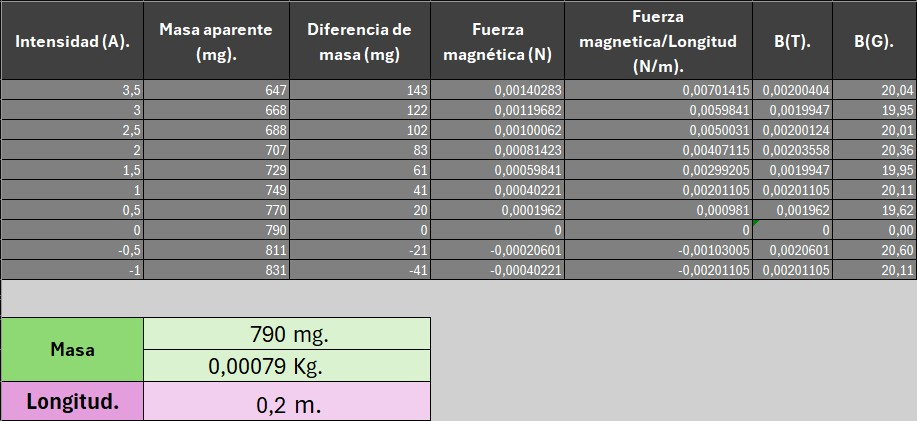
\includegraphics[width=0.9\textwidth]{fig13.jpg}
    \caption{Una vez tomamos los datos, procedemos a obtener los demás datos como \textbf{Diferencia de masa, Fuerza magnética, Campos magnéticos y el campo como resultado de la fuerza partida la longitud.}}
\end{figure}

\subsection{Ajuste Lineal.}

\begin{figure}[H]
	\centering
	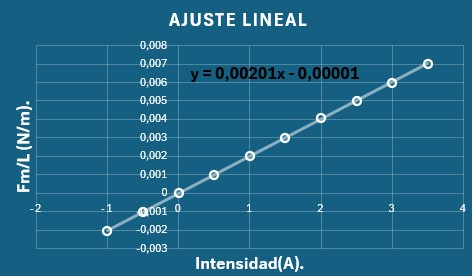
\includegraphics[width=0.9\textwidth]{fig14.jpg}
    \caption{Una vez con los datos, graficamos el ajuste lineal donde al igual que en la primera imagen (la simulación) obtenemos la ecuación de la pendiente y el valor del campo magnético en (G). }
\end{figure}

\section{Revisión.}


\begin{figure}[H]
	\centering
	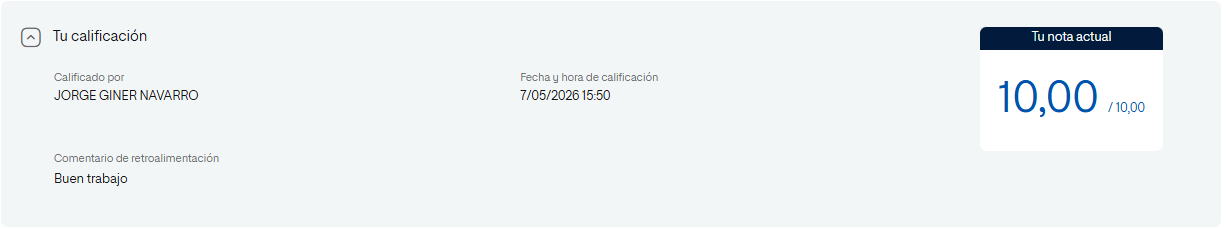
\includegraphics[width=1.2\textwidth]{revision.png}
\end{figure}

\end{document}